\section{Observations}
\label{sec:observations}

\subsection{Key Similarity}

High cosine similarity between adjacent key states has been observed and studied in KVMerger~\citep{wang2024kvmerger}.
They derive a theoretical lower bound on the cosine similarity between key vectors at positions $n$ and $m$ of $\cos(n - m)$, which puts the minimum similarity of any adjacent pair at $\cos(1) \approx 0.54$.
As the distance between tokens grows, the bound decreases toward zero.
Since this pattern does not appear in value states, they attribute the phenomenon entirely to RoPE.

In this section we look at the pre-RoPE key states to check whether other factors also contribute.
We feed LLaMA-3 8B Instruct a sequence of 512 tokens sampled from WikiText-103 and record key states at layers 0, 8, 16, and 23.
At each layer we compute the average cosine similarity between all adjacent token pairs and average over heads.
We repeat this for five configurations:

\begin{enumerate}
    \item \textbf{pre-RoPE real}: key states before RoPE, original token order
    \item \textbf{pre-RoPE shuffled}: key states before RoPE, token positions randomly shuffled
    \item \textbf{post-RoPE real}: key states after RoPE, original token order
    \item \textbf{post-RoPE content-shuffled}: input sequence shuffled before keys are computed, RoPE applied in natural positional order
    \item \textbf{post-RoPE key-shuffled}: key states after RoPE, token positions randomly shuffled
\end{enumerate}

\begin{figure}[!ht]
    \centering
    
\includegraphics[width=\linewidth]{../assets/cos_analysis.png}
    \caption{Average cosine similarity of adjacent key states under five configurations for LLaMA-3 8B Instruct at layers 0, 8, 16, and 23.}
    \label{fig:cos_analysis}
\end{figure}

Configuration 2 in Figure~\ref{fig:cos_analysis} (pre-RoPE shuffled) already shows high cosine similarity.
Since the token order is random here, neither positional encoding nor content adjacency can explain it.
The key projection itself pushes key states into a narrow region of the key space, raising the global similarity.
This is the structure that low-rank KV compression methods exploit, such as EigenAttention~\citep{saxena2024eigenattention} and DeepSeek MLA~\citep{deepseekai2024deepseekv2}.

In mid and deep layers, configuration 1 (pre-RoPE real) in Figure~\ref{fig:cos_analysis} shows noticeably higher similarity than configuration 2.
Adjacent tokens in natural text tend to be semantically related, and this is reflected in their key states.

Comparing configurations 1 and 3 in Figure~\ref{fig:cos_analysis} (pre- and post-RoPE on the real sequence), the similarity values are nearly identical.
When content is in natural order, applying RoPE does not significantly change adjacent token similarity.

Configuration 4 in Figure~\ref{fig:cos_analysis} shows a different picture.
The input content is shuffled before keys are computed, so the key states lack content-driven adjacency.
After RoPE is applied, the similarity recovers to nearly the level of configuration 3.
RoPE raises the similarity of adjacent positions regardless of the underlying content order.

Configuration 5 in Figure~\ref{fig:cos_analysis} (post-RoPE key-shuffled) shows what happens if we break positional adjacency after RoPE is applied. The similarity drops back down, confirming that RoPE's contribution relies on evaluating adjacent positions sequentially.

Key similarity at the token level is therefore a combination of three factors: the key projection creates a high global similarity floor, semantic content raises similarity further for adjacent tokens in natural text, and RoPE contributes a positional adjacency structure on top of that.

\subsection{Query Similarity}

The same analysis on query states shows that the query projection has the same properties as the key projection.
Query vectors show high cosine similarity regardless of token order, which means the projection itself pushes queries into a narrow region of the query space.
In later layers, similarity is higher for real sequences than for shuffled ones, suggesting that query vectors pick up contextual information and adjacent tokens in natural text end up closer together.
As with keys, applying RoPE to shuffled sequences (post-RoPE content-shuffled) recovers adjacent similarity, contributing a positional structure on top of the content signal. Furthermore, breaking the positional adjacency after RoPE (post-RoPE Q-shuffled) drops the similarity back down.

\begin{figure}[!ht]
    \centering
    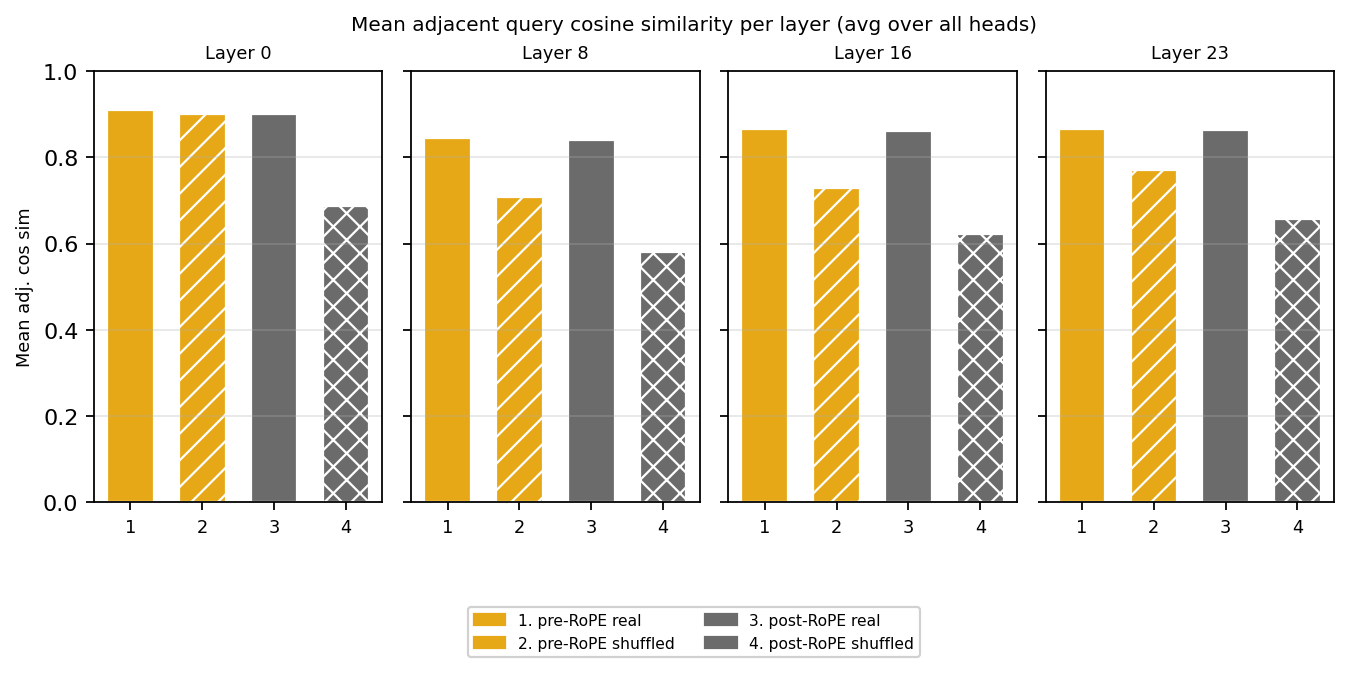
\includegraphics[width=\linewidth]{../assets/query_similarity_mean_by_layer.png}
    \caption{Mean adjacent query cosine similarity per layer (averaged over all heads) for LLaMA-3 8B Instruct at layers 0, 8, 16, and 23, under five configurations: pre-RoPE real, pre-RoPE shuffled, post-RoPE real, post-RoPE content-shuffled, and post-RoPE Q-shuffled.}
    \label{fig:query_similarity}
\end{figure}
